\documentclass[12pt,a4paper,openright,twoside]{book}
\usepackage[utf8]{inputenc}
\usepackage{disi-thesis}
\usepackage{code-lstlistings}
\usepackage{notes}
\usepackage{shortcuts}
\usepackage{acronym}
\school{\unibo}
\programme{Corso di Laurea Magistrale in Ingegneria e Scienze Informatiche}
\title{Fancy Title}
\author{Giacomo Accursi}
\date{\today}
\subject{Laboratorio di Sistemi Software}
\supervisor{Prof. Danilo Pianini}
\cosupervisor{Dott. Gianluca Aguzzi}
\session{IV}
\academicyear{2022-2023}

% Definition of acronyms
% \acrodef{IoT}{Internet of Thing}
% \acrodef{vm}[VM]{Virtual Machine}


\mainlinespacing{1.241}

\begin{document}

\frontmatter\frontispiece

\begin{abstract}	
Max 2000 characters, strict.
\end{abstract}

\begin{dedication} % this is optional
Optional. Max a few lines.
\end{dedication}

\begin{acknowledgements} % this is optional
Optional. Max 1 page.
\end{acknowledgements}

%----------------------------------------------------------------------------------------
\tableofcontents   
\listoffigures     % (optional) comment if empty
\lstlistoflistings % (optional) comment if empty
%----------------------------------------------------------------------------------------

\mainmatter

%----------------------------------------------------------------------------------------
\chapter{Introduzione}
\label{chap:introduzione}
%----------------------------------------------------------------------------------------

% Write your intro here.
% \sidenote{Add sidenotes in this way. They are named after the author of the thesis}

% You can use acronyms that your defined previously,
% such as \ac{IoT}.
% %
% If you use acronyms twice,
% they will be written in full only once
% (indeed, you can mention the \ac{IoT} now without it being fully explained).
% %
% In some cases, you may need a plural form of the acronym.
% %
% For instance,
% that you are discussing \acp{vm},
% you may need both \ac{vm} and \acp{vm}.

% \paragraph{Structure of the Thesis}

% \note{At the end, describe the structure of the paper}

% \chapter{State of the art}

% I suggest referencing stuff as follows: \cref{fig:random-image} or \Cref{fig:random-image}


% \section{Some cool topic}

% \chapter{Contribution}

% You may also put some code snippet (which is NOT float by default), eg: \cref{lst:random-code}.

% \lstinputlisting[float,language=Java,label={lst:random-code}]{listings/HelloWorld.java}


%----------------------------------------------------------------------------------------
% Discrete Event Simulation
%----------------------------------------------------------------------------------------
\chapter{Simulazioni ad Eventi Discreti}
\section{Panoramica sulle simulazioni ad eventi discreti}
\label{sec:panoramica-des}
Un sistema ad eventi discreti è un sistema a stati discreti guidato da eventi, il cui il progresso del tempo è determinato dall'occorrenza di eventi grazie ai quali il sistema evolve. Nel contesto di una simulazione ad eventi discreti, un evento rappresenta un cambiamento nello stato del sistema. 
Gli esempi di eventi possono includere l'arrivo di un messaggio in un sistema di comunicazione, il completamento di un processo, o qualsiasi altro avvento che influenzi il comportamento del sistema. La simulazione avanza di passi discreti, con ogni passo che corrisponde all'accadimento di un nuovo evento. 
Questo approccio è spesso utilizzato per modellare e analizzare sistemi complessi, come reti di computer, catene di approvvigionamento, code di attesa o altri scenari in cui gli eventi guidano il comportamento del sistema. 

\subsection{Terminologia e componenti}
I concetti alla base di un sistema ad eventi discreti sono i seguenti: 
\begin{itemize}
    \item \textbf{Sistema}: collezione di entità che interagiscono fra loro nel tempo per raggiungere determinati obiettivi.
    \item \textbf{Modello}: una rappresentazione astratta del sistema, spesso contenente relazioni strutturali, logiche o matematiche che descrivono il sistema stesso.
    \item \textbf{Stato del sistema}: una collezione di variabili che contengono tutte le informazioni necessarie per descrivere il sistema in ogni momento.
    \item \textbf{Entità}: un oggetto nel sistema che richiede una rappresentazione esplicita nel modello. Le entità possono essere create in fase di inizializzazione della simulazione o durante essa. 
    \item \textbf{Attributi}: sono le proprietà di una determinata entità.
    \item \textbf{Evento}: una occorrenza istantanea che cambia lo stato del sistema. 
    \item \textbf{Lista degli eventi futuri (FEL)}: contiene tutti gli eventi futuri ordinati cronologicamente in base al tempo di accadimento. Deve essere implementata in modo che gestisca in maniera efficiente l'aggiunta, la rimozione e la ricerca di eventi. 
    \item \textbf{Clock}: una variabile rappresentante il tempo simulato. In generale non esiste nessuna correlazione fra il tempo simulato e il tempo necessario per eseguire la simulazione. 
\end{itemize}
Una simulazione ad eventi discreti procede acquisendo una sequenza di \textit{snapshot}, i quali rappresentano l'evoluzione del sistema nel tempo. Uno snapshot ad un determinato istante $t$, include non solo lo stato del sistema al tempo $t$, ma anche la lista degli eventi futuri e lo stato di tutte le entità del sistema.

\subsection{Algoritmo Event-scheduling Time-advance}
\label{sec:time-advance-algorithm}
La dinamicità intrinseca delle simulazioni ad eventi discreti impone la necessità di gestire attentamente il flusso temporale attraverso il monitoraggio costante del clock. 
Un meccanismo fondamentale per garantire l'evoluzione accurata della simulazione, rispettando l'ordine cronologico degli eventi, è rappresentato dall'algoritmo ``\textit{event-scheduling time-advance}'', basato sull'utilizzo della future event list (FEL).

\begin{figure}
    \centering
    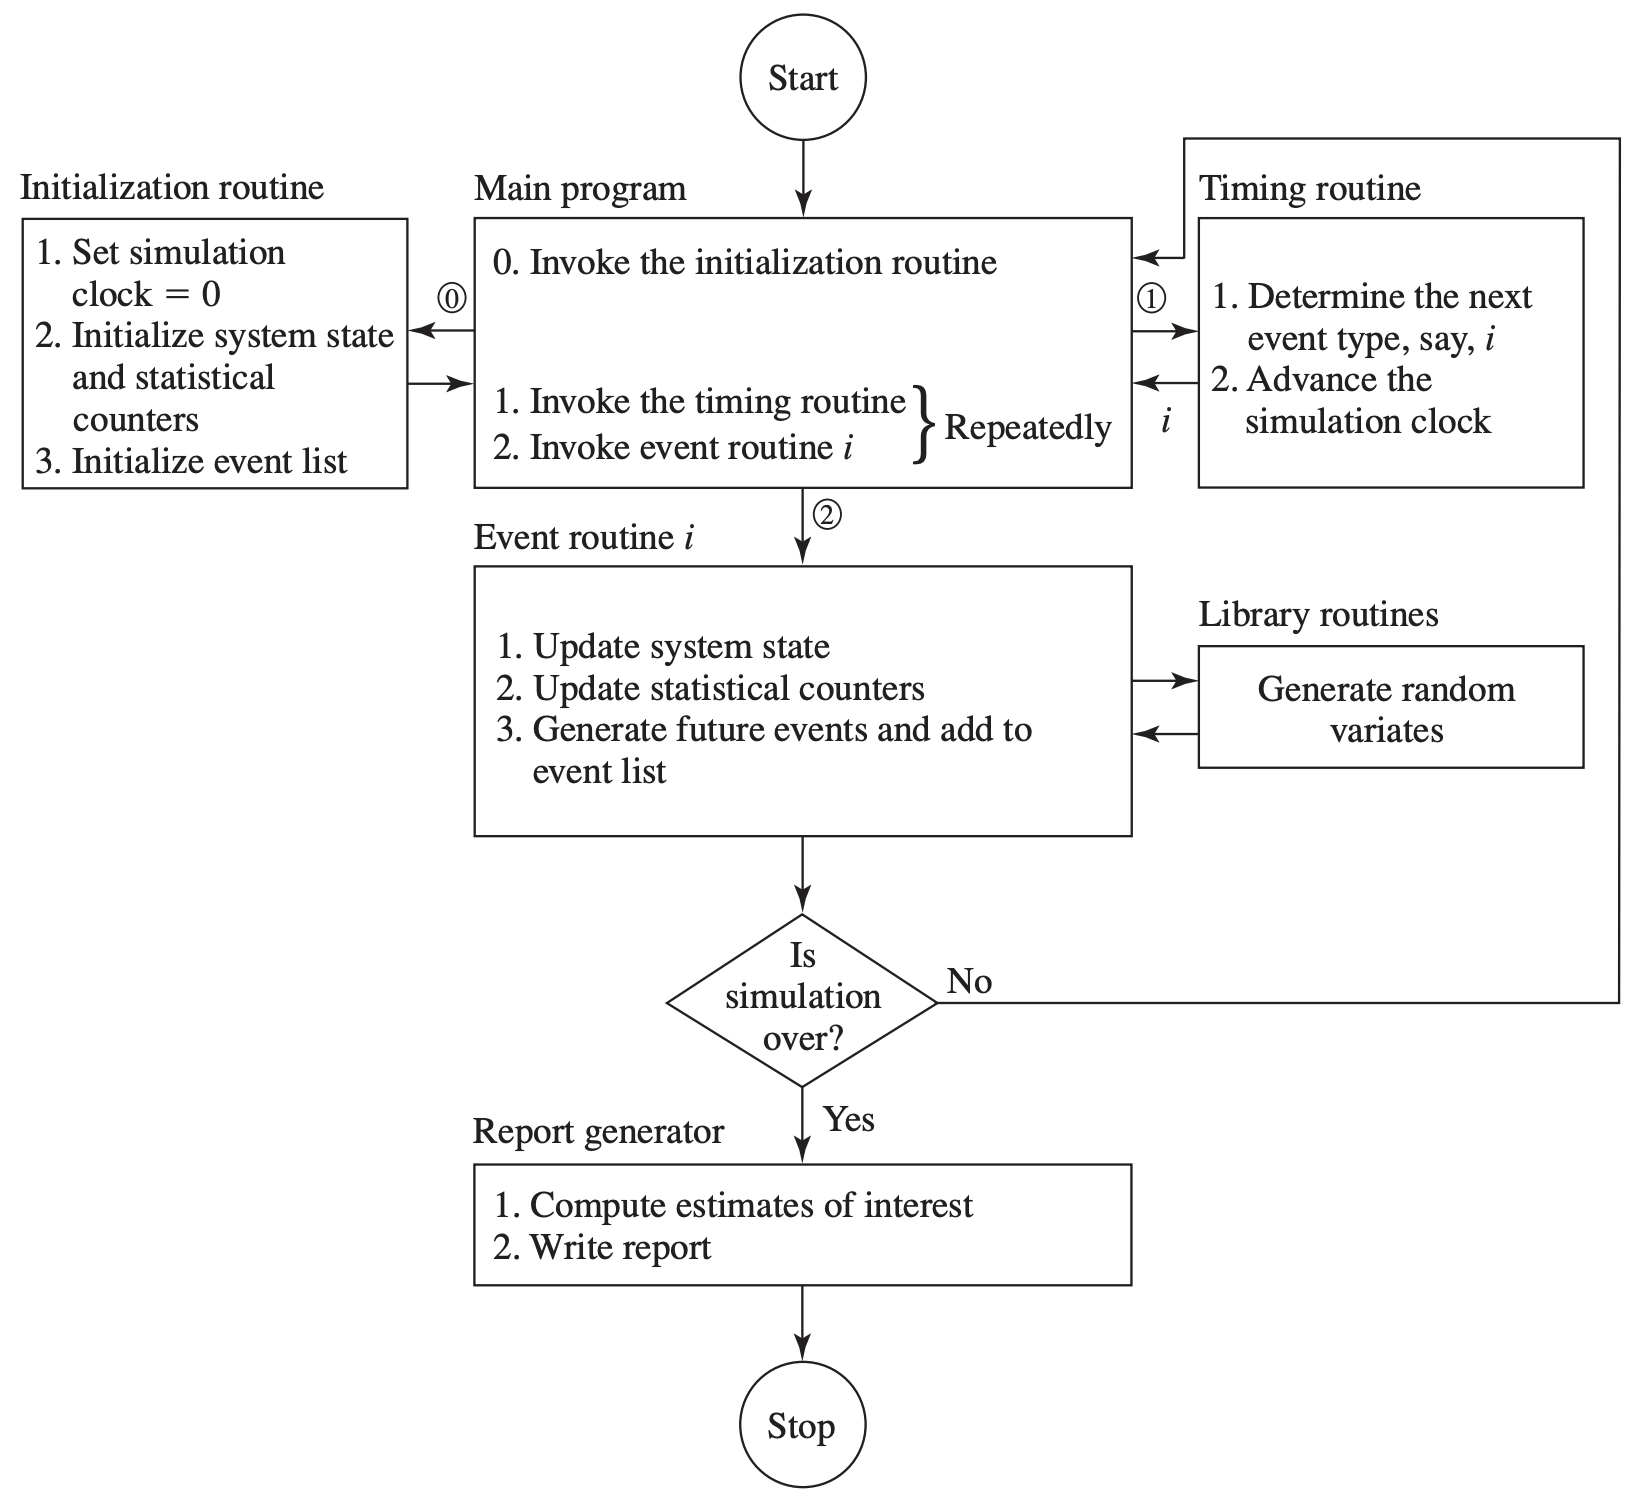
\includegraphics[width=.80\linewidth]{figures/discrete-event-simulation/time-advance-flow.png}
    \caption{Flusso di controllo dell'algoritmo event-scheduling time-advance \cite{Law15}.}
    \label{fig:next-event-flow}
\end{figure}

L'algoritmo in questione, il cui flusso di controllo è illustrato in figura~\ref{fig:next-event-flow}, è suddiviso in tre sezioni chiave: \textit{inizializzazione}, \textit{ciclo di elaborazione degli eventi} e \textit{fase di output}.
La simulazione inizia al tempo 0, quando il \textit{main program} dà avvio alla simulazione invocando la \textit{initialization routine}, nella quale il clock viene settato a 0 e le entità e le variabili di stato sono inizializzate.
Il controllo torna poi al main program, il quale invoca una \textit{timing routine} per identificare il prossimo evento da eseguire.
La lista degli eventi futuri contiene tutti gli eventi ordinati per tempo di accadimento: $FEL = [t_1, t_2, \dots t_n], t_1 \leq t_2 \leq \dots \leq t_n$. 
Il tempo $t$ è il valore corrente del clock, mentre l'evento associato al tempo $t_1$ è chiamato evento imminente, ovvero il prossimo evento che dovrà verificarsi~\cite{DBLP:books/daglib/0034857}.
Il controllo torna nuovamente al \textit{main program}, il quale invoca l'\textit{event routine} grazie al quale l'evento imminente viene eseguito effettivamente. 
L'esecuzione dell'evento imminente, seguita dalla generazione di uno snapshot correlato, comporta l'avanzamento del clock al successivo istante temporale. L'evento imminente è rimosso quindi dalla FEL ed eseguito, generando un nuovo snapshot al tempo $t_1$ basato sulla natura dell'evento e lo snapshot precedente. In questa fase nuovi eventi futuri possono essere generati e aggiunti opportunamente alla FEL.
Il processo si ripete ciclicamente fino alla conclusione della simulazione. 
Durante la fase di output vengono invece elaborate e registrate le statistiche di interesse. 

\subsubsection{Gestione Future Event List}
Una Future Event List, come anticipato, è la struttura dati che contiene l'elenco degli eventi programmati per verificarsi in futuro. Tradizionalmente l'elenco è ordinato in base al tempo di esecuzione al quale l'evento è stato schedulato, ma questo non è un requisito. 
La gestione efficiente della FEL è di fondamentale importanza, alcuni modelli di simulazione impiegano più tempo CPU nella gestione della lista piuttosto che qualsiasi altro aspetto, come per esempio la generazione di numeri casuali, l'elaborazione di eventi, l'esecuzione di operazioni aritmetiche varie ecc\dots

Nella gestione degli eventi che compongono la FEL, ci sono due operazioni critiche: l'operazione di inserimento (\textit{enqueue}) e l'operazione di cancellazione (\textit{dequeue}). Un'operazione di cancellazione viene eseguita per elaborare l'evento o perché un evento, precedentemente pianificato deve essere annullato per qualche motivo. L'inserimento e la cancellazione possono verificarsi in una posizione prescritta nella lista degli eventi, oppure potrebbe essere necessario avviare una ricerca per determinare la giusta posizione. 
Importante è anche l'operazione di modifica, in cui una ricerca di evento esistente presente in lista è seguita da una modifica di qualche aspetto dell'evento stesso, come ad esempio la modifica del tempo di accadimento al quale è schedulato. 

Esistono tre criteri principali per determinare l'efficacia della struttura dati e dell'algoritmo per la gestione della FEL: 
\begin{itemize}
    \item \textbf{velocità}: la struttura dati e l'algoritmo per inserire ed eliminare un evento devono essere ottimizzate per minimizzare il tempo di esecuzione. Per ottenere tempi di esecuzione rapidi è fondamentale una ricerca degli eventi efficiente. Un algoritmo efficiente tende a limitare il numero di eventi ricercati per l'inserimento o la cancellazione;
    \item  \textbf{robustezza}: è necessaria una gestione efficace degli errori per affrontare scenari imprevisti. Occorre una validazione dei dati durante l'inserimento per garantire l'integrità della struttura dati; 
    \item \textbf{adattabilità}: la FEL dovrebbe consentire la configurazione di parametri chiave per adattarsi a diverse modalità di gestione degli eventi o politiche temporali. Dovrebbe inoltre essere progettata in modo che nuove funzionalità o tipi di eventi possano essere facilmente integrati senza modificare drasticamente il codice esistente. 
\end{itemize}

\subsection{Partenza e terminazione}
Nella \Cref{sec:time-advance-algorithm} è stato descritto come la simulazione avanza durante la sua esecuzione. Tipicamente per far partire una simulazione, in fase di inizializzazione viene generato un evento specifico che viene poi inserito nella lista di eventi futuri. 
La terminazione può invece essere raggiunta tramite diversi meccanismi: 
\begin{itemize}
    \item tempo di simulazione massimo: al tempo 0 viene schedulato un evento di stop ad un tempo futuro $T_e$. In questo caso siamo certi che la simulazione verrà eseguita nell'intervallo $[0, T_e]$; 
    \item eventi speciali di terminazione: il tempo di esecuzione $T_e$ è determinato dalla simulazione stessa. In genere $T_e$ dipende dal numero di occorrenze di un determinato evento. Per esempio potrebbe essere il tempo del completamento del centesimo servizio presso un determinato centro di assistenza;  
    \item terminazione quando la FEL è vuota.
\end{itemize}
Nel secondo e nel terzo caso il tempo per eseguire la simulazione non è conosciuto a priori e può variare di simulazione in simulazione.
Le esecuzioni di una simulazione possono essere classificate in \textit{transient} e \textit{steady state}. La selezione del tipo di simulazione è particolarmente importante e la decisione deve essere presa in base all'output che vogliamo analizzare. Con il termine \textit{transient} ci si riferisce ad una simulazione che termina, per causa di un evento speciale o grazie ad un tempo prefissato. 
Una simulazione \textit{steady state}, al contrario, non termina mai. L'obiettivo in questo caso è studiare il comportamento a lungo termine del sistema. 

\subsection{Distribuzioni di probabilità}
Il successo di una simulazione richiede un approccio completo che va oltre la semplice creazione di un diagramma di flusso del sistema in esame, la sua traduzione in un ``programma'' per computer e la replicazione di alcune configurazioni proposte del sistema. L'uso della probabilità e della statistica è un aspetto fondamentale di uno studio di simulazione, tanto che ogni team di modellazione dovrebbe includere almeno un esperto con una solida formazione in queste tecniche~\cite{Law15}.
Per effettuare una simulazione, utilizzando input casuali come i tempi di arrivo o le dimensioni della domanda, occorre specificare le loro distribuzioni di probabilità. La scelta delle corrette distribuzioni determina in maniera importante l'accuratezza del modello. 

Nelle simulazioni ad eventi discreti è comune modellare il tempo trascorso tra gli arrivi successivi degli eventi utilizzando distribuzioni di probabilità. 
Ad esempio, nel caso di una coda di attesa in un sistema di servizio, i tempi tra gli arrivi dei clienti possono essere modellati utilizzando una distribuzione esponenziale o di Poisson. Queste distribuzioni consentono di rappresentare realisticamente il processo di arrivo degli eventi e di stimare la frequenza con cui si verificano.
I tempi di servizio potrebbero essere invece costanti o probabilistici. Se i tempi sono completamente casuali, potrebbe essere necessario dover utilizzare una distribuzione esponenziale. Potrebbe anche accadere che i tempi di servizio siano costanti, ma una variabilità casuale causi fluttuazioni in modo negativo o positivo. Ad esempio, il tempo impiegato da un tornio per attraversare un albero di 10 centimetri dovrebbe essere costante. Tuttavia, il materiale potrebbe presentare lievi differenze di durezza o lo strumento potrebbe usurarsi. Qualsiasi evento potrebbe causare tempi di lavorazione diversi. In questi casi la distribuzione normale potrebbe descrivere il tempo di servizio~\cite{DBLP:books/daglib/0034857}.
Oltre ai tempi di arrivo e di servizio, le simulazioni possono coinvolgere altre variabili casuali che influenzeranno il comportamento del sistema: i ritardi tra l'arrivo di un evento e la sua elaborazione possono essere modellati utilizzando distribuzioni di probabilità per rappresentare il tempo impiegato per completare determinate attività o processi. 

\subsection{Simulazione parallela}
La simulazione parallela a eventi discreti (PDES) si riferisce all'esecuzione di un singolo programma di simulazione a eventi discreti su un computer sfruttando il calcolo parallelo~\cite{DBLP:journals/cacm/Fujimoto90}. Distribuendo l'esecuzione di una simulazione su più processori, si cerca di ridurre notevolmente il tempo di esecuzione del modello, fino a un fattore pari al numero di processori. Questo concetto è valido in teoria, in realtà la legge di Amdahl stabilisce che il miglioramento della velocità di esecuzione di un programma parallelizzabile su un sistema multi-core è limitato dalla frazione sequenziale del programma~\cite{DBLP:conf/afips/Amdahl67}. In altra parole, anche se una parte del programma può essere eseguita in modo parallelo, ci sarà sempre una parte sequenziale che non può essere parallelizzata. La legge di Amdahl può essere espressa con la seguente formula: 
$$
Speedup_{max} = \frac{1}{(1-P)+\frac{P}{N}}
$$
Dove: 
\begin{itemize}
    \item $Speedup_{max}$ è il miglioramento massimo della velocità di esecuzione ottenibile parallelizzando il programma. 
    \item $P$ è la frazione di codice che può essere parallelizzata. 
    \item $N$ è il numero di core disponibili.
\end{itemize}

Se si sta simulando un modello militare di grandi dimensioni o una rete di comunicazione contenente migliaia di nodi, il tempo di esecuzione potrebbe essere eccessivo e si potrebbe prendere in considerazione la simulazione parallela. Un altro uso della simulazione parallela potrebbe essere il processo decisionale in tempo reale. Ad esempio, in un sistema di controllo del traffico aereo, potrebbe risultare utile simulare diverse ore di traffico aereo per decidere come reindirizzarlo al meglio~\cite{DBLP:conf/wsc/Wieland98}. 

Lo sviluppo di una simulazione parallela richiede la scomposizione del modello in processi logici (LP). I singoli LP sono assegnati a processori diversi, ognuno dei quali si occupa di simulare la propria parte di modello. Gli LP comunicano fra loro inviandosi messaggi o eventi con data e ora.
Quando si progetta una simulazione parallela è di fondamentale importanza garantire che gli eventi del modello, indipendentemente dal loro LP, vengano elaborati nella corretta sequenza temporale, mantenendone in questo modo l'ordine causale. Se ogni LP elabora tutti i suoi eventi (generati da se stesso o da un altro LP) in ordine di tempo crescente, garantendo che gli eventi successivi siano eseguiti solo dopo quelli precedenti, e garantendo che gli eventi siano correttamente sincronizzati durante l'esecuzione in parallelo, allora l'ordine causale viene automaticamente conservato nella simulazione distribuita. Questo principio è cruciale per evitare inconsistenze e risultati non realistici.
Ogni LP può essere visto come un modello di simulazione sequenziale a eventi discreti, con le proprie variabili di stato locali, i propri eventi e il proprio clock.

Storicamente sono stati adottati due meccanismi di sincronizzazione differente: \textit{conservativo} e \textit{ottimistico}~\cite{DBLP:conf/wsc/Fujimoto95}.
Quando si utilizza un meccanismo conservativo l'obiettivo è evitare di violare il vincolo di causalità temporale. Ad esempio, si supponga che un particolare LP si trovi attualmente al tempo di simulazione 25 e sia pronto a elaborare il prossimo evento, che ha un tempo di 30. Il meccanismo di sincronizzazione deve assicurarsi che questo LP non riceva in seguito un evento da un altro LP con tempo di accadimento inferiore a 30. Pertanto, l'obiettivo è determinare quando è effettivamente sicuro elaborare un particolare evento. 
La sincronizzazione conservativa presenta due principali svantaggi: 
\begin{itemize}
    \item non può sfruttare appieno il parallelismo disponibile: se l'evento A influenza in qualche modo l'evento B, allora A e B devono essere eseguiti in sequenza. Se il modello è tale per cui A influisce raramente B, allora A e B potrebbero essere elaborati in modo concorrente per la maggior parte del tempo;
    \item non è robusta: una modifica apparentemente piccola del modello può inficiare le prestazioni. 
\end{itemize}
Nella sincronizzazione di tipo ottimistico, le violazioni del vincolo di causalità locale possono verificarsi, ma il meccanismo di sincronizzazione rileva le violazioni e le recupera. Anche in questo caso ogni LP simula la propria porzione di modello in avanti nel tempo, ma non aspetta di ricevere messaggi da altri processi. 
Il meccanismo \textit{time-warp}~\cite{DBLP:journals/toplas/Jefferson85} è il più noto approccio ottimistico. Se un LP riceve un messaggio che avrebbe dovuto ricevere nel suo passato (e che quindi potrebbe influenzare le sue azioni da quel momento in poi), viene effettuato un \textit{rollback} nell'LP ricevente che porta il suo clock all'ora del messaggio in arrivo.
Parte del lavoro annullato potrebbe consistere nell'invio di messaggi ad altri LP. L'invio di questi messaggi viene anch'esso annullato grazie all'invio del corrispondente anti-messaggio. L'invio di anti-messaggi può generare a sua volta rollback secondari negli LP di destinazione.
I meccanismi di sincronizzazione ottimistici possono sfruttare il parallelismo in modo migliore rispetto agli approcci conservativi, poiché non sono limitati dallo scenario peggiore. Tutta via presentano comunque alcuni svantaggi: 
\begin{itemize}
    \item comportano costi computazionali maggiori legati all'esecuzione dei rollback; 
    \item per poter effettuare i rollback lo stato di ogni LP deve essere salvato periodicamente, comportando un maggiore utilizzo di memoria.
\end{itemize}


\subsection{Cenni Storici}
La storia delle simulazioni ad eventi discreti si estende per oltre mezzo secolo, risalendo ai primi anni dell'era informatica. La necessità di modellare e comprendere il comportamento dinamico dei sistemi complessi spinse i ricercatori a sviluppare metodologie e strumenti per simulare il funzionamento di tali sistemi.

Le radici concettuali delle simulazioni ad eventi discreti possono essere rintracciate nella teoria dei processi stocastici, che ha trovato applicazioni pratiche nell'ambito dell'ingegneria, della gestione delle operazioni aziendali e della logistica. Nel corso degli anni '50 e '60, con l'avvento dei primi computer e l'espansione dei linguaggi di programmazione, emersero i primi tentativi di simulare sistemi complessi utilizzando modelli basati su eventi discreti. Questi primi sforzi furono spesso limitati dalle risorse computazionali disponibili e dalle limitazioni dei linguaggi di programmazione dell'epoca.
Negli anni '60 e '70, con l'avanzamento della tecnologia informatica e l'introduzione di linguaggi di programmazione più potenti, come FORTRAN e ALGOL, la simulazione ad eventi discreti divenne sempre più praticabile e diffusa. Durante questo periodo furono sviluppati i primi linguaggi di programmazione specificamente progettati per la simulazione, come SIMSCRIPT~\cite{DBLP:journals/ibmsj/DimsdaleM64} e GPSS~\cite{DBLP:journals/tssc/HollandM68}, i quali permisero ai ricercatori di modellare e analizzare sistemi complessi in modo più efficace e efficiente.

Negli anni successivi, con il continuo avanzamento della tecnologia informatica e l'introduzione di nuovi concetti e metodologie, come la simulazione ad oggetti e la simulazione basata su agenti, le simulazioni ad eventi discreti continuarono ad evolversi e a trovare sempre più applicazioni in una vasta gamma di settori. 
Molte aziende, in particolare nel settore manifatturiero, utilizzarono le simulazioni come strumento di supporto alle decisioni. 

A livello informatico il nuovo millennio è stato caratterizzato dalla potenza sempre crescente dei personal computer, dalla diminuzione del prezzo di questi ultimi e dal World Wide Web~\cite{DBLP:journals/jors/Robinson05}. Le simulazioni hanno cominciato a integrare intelligenza artificiale e machine learning per migliorare la previsione e l'ottimizzazione dei sistemi. Inoltre, la crescente disponibilità di dati in tempo reale ha portato all'adozione di approcci di simulazione ibrida che combinano modelli ad eventi discreti con dati reali per migliorare la precisione delle previsioni e delle decisioni.


\subsection{Aree di impiego}

L'adozione delle simulazioni ad eventi discreti riveste un ruolo cruciale in numerose aree di studio e applicazioni pratiche, offrendo un metodo efficace per esplorare e comprendere il comportamento dei sistemi complessi. Attraverso l'utilizzo di modelli matematici e algoritmi appropriati, le simulazioni ad eventi discreti consentono di esaminare scenari variabili, prendendo in considerazione la casualità e la complessità intrinseche dei processi reali.
In vari ambiti l'adozione di simulazioni ad eventi discreti offre numerosi vantaggi. Queste simulazioni consentono di valutare strategie, ottimizzare processi, identificare aree di miglioramento e prevedere l'andamento futuro dei sistemi analizzati. Grazie alla possibilità di eseguire esperimenti virtuali ripetibili e controllati, le simulazioni ad eventi discreti permettono agli operatori e agli studiosi di testare diverse ipotesi e strategie senza dover intervenire direttamente sui sistemi reali, riducendo così i costi e i rischi associati all'implementazione di nuove soluzioni.

\subsubsection{Sistemi di Produzione e Movimentazione dei Materiali}
I sistemi di produzione e movimentazione dei materiali rappresentano una delle applicazioni più importanti della simulazione. La simulazione è stata utilizzata con successo come supporto nella progettazione di nuove strutture produttive, magazzini e centri di distribuzione.
Le simulazioni ad eventi discreti sono utilizzate per condurre analisi sulla capacità di produzione degli impianti, considerando le specifiche delle risorse disponibili come macchinari, manodopera e materiali. Questo aiuta ad individuare sovraccarichi o sottoutilizzazioni delle risorse e a pianificare la capacità in modo efficiente. 
Oltre alla produzione, viene impiegata anche per ottimizzare la logistica, comprese le operazioni di movimentazione dei materiali, lo stoccaggio, il prelievo, il trasporto e la distribuzione. Questo comprende l'analisi della disposizione degli impianti, dei percorsi di movimentazione e delle politiche di gestione degli inventari per massimare l'efficienza complessiva e ridurre i costi operativi. 
I simulatori ad eventi discreti consentono di modellare anche i sistemi di trasporto e distribuzione dei materiali sia all'interno che all'esterno dell'impianto manifatturiero. Ciò include la pianificazione delle rotte di trasporto, l'ottimizzazione dei tempi di consegna e l'analisi dei flussi di traffico per garantire una distribuzione efficiente dei materiali.
Infine, è possibile valutare le performance attuali del sistema di produzione e movimentazione dei materiali e testare strategie di miglioramento. Questo può includere l'implementazione di nuove tecnologie, l'ottimizzazione dei processi o la riduzione degli sprechi, contribuendo a migliorare complessivamente l'efficienza e la produttività del sistema.


\subsubsection{Sistemi informatici}
La simulazione dei sistemi informatici consente di modellare e analizzare il comportamento di reti di computer, server e sistemi distribuiti. 
I simulatori possono essere utilizzati per valutare le prestazioni del sistema, misurare latenza di rete, analizzare il throughput e identificare eventuali bottleneck. Inoltre, consentono di simulare il carico di lavoro sui sistemi, aiutando a ridimensionare correttamente l'infrastruttura e a pianificare l'allocazione di risorse. 
È possibile simulare anche l'utilizzo di nuovi algoritmi o politiche di gestione delle risorse, come strategie di scheduling dei processi e politiche di gestione della memoria.
Modellare scenari di fallimento e valutare l'impatto dei guasti, valutando l'impatto di questi ultimi sulle prestazioni del sistema e sulla disponibilità dei servizi, consente di valutare la tolleranza ai guasti di sistemi informatici complessi. 
Anche la sicurezza del sistema può essere valutata, simulando scenari di minaccia e attacchi informatici, così da identificare eventuali vulnerabilità.

\subsubsection{Reti Informatiche}
La simulazione di reti informatiche consente di comprendere il comportamento dinamico delle reti e consente di valutare le prestazioni di quest'ultima, misurando parametri chiave come la \textit{latenza} e il \textit{throughput}. Questo permette di identificare e risolvere eventuali punti critici che potrebbero compromettere le prestazioni della rete. 
Studiando il traffico di rete è possibile individuare possibili congestioni di rete e adottare strategie di routing per garantire una gestione efficiente delle risorse. 
Un altro aspetto importante è la possibilità di valutare la scalabilità della rete, ovvero la sua capacità di gestire un aumento del carico di lavoro o del numero di utenti. 
Il testing di nuovi protocolli e tecnologie consente di valutare le prestazioni di nuove soluzioni prima della loro effettiva implementazione su larga scala. 
Anche in questo caso, modellando scenari di attacco e valutando la robustezza delle contromisure di sicurezza adottate, è possibile analizzare la sicurezza della rete, proteggendola da minacce esterne e garantendo la sicurezza dei dati sensibili. 

\section{Simulazioni ad eventi discreti vs continue}
Ogni modello di simulazione è la specifica di un sistema fisico (o una parte di esso) in termini di un insieme di stati ed eventi. 
Effettuare una simulazione significa imitare l'occorrenza degli eventi che evolvono nel tempo e riconoscerne gli effetti, rappresentati come stati~\cite{PDES}. 
Gli eventi futuri indotti dagli stati devono essere pianificati. Come è possibile notare in~\Cref{fig:Continuous-vs-Discrete} in una simulazione continua i cambiamenti di stato avvengono continuamente nel tempo, mentre in una simulazione discreta il verificarsi di un evento è istantaneo e limitato a un punto selezionato nel tempo. 
Il concetto di tempo continuo modella il tempo come un continuum di punti temporali successivi. Questo implica che i dati forniti per un certo arco di tempo sono specificati come una funzione continua nel tempo. In genere si assume che questa funzione sia anche differenziabile, in modo che che le variazioni della variabile di stato nel tempo possano essere modellate come la derivata prima della variabile di stato. Gli intervalli di tempo non svolgono un ruolo specifico come principio organizzativo. Naturalmente si può considerare qualsiasi intervallo di tempo, ma non intervalli di tempo predefiniti di lunghezza finita che strutturano l'intero modello~\cite{Ossimitz2008TheBO}. 
\begin{figure}
    \centering
    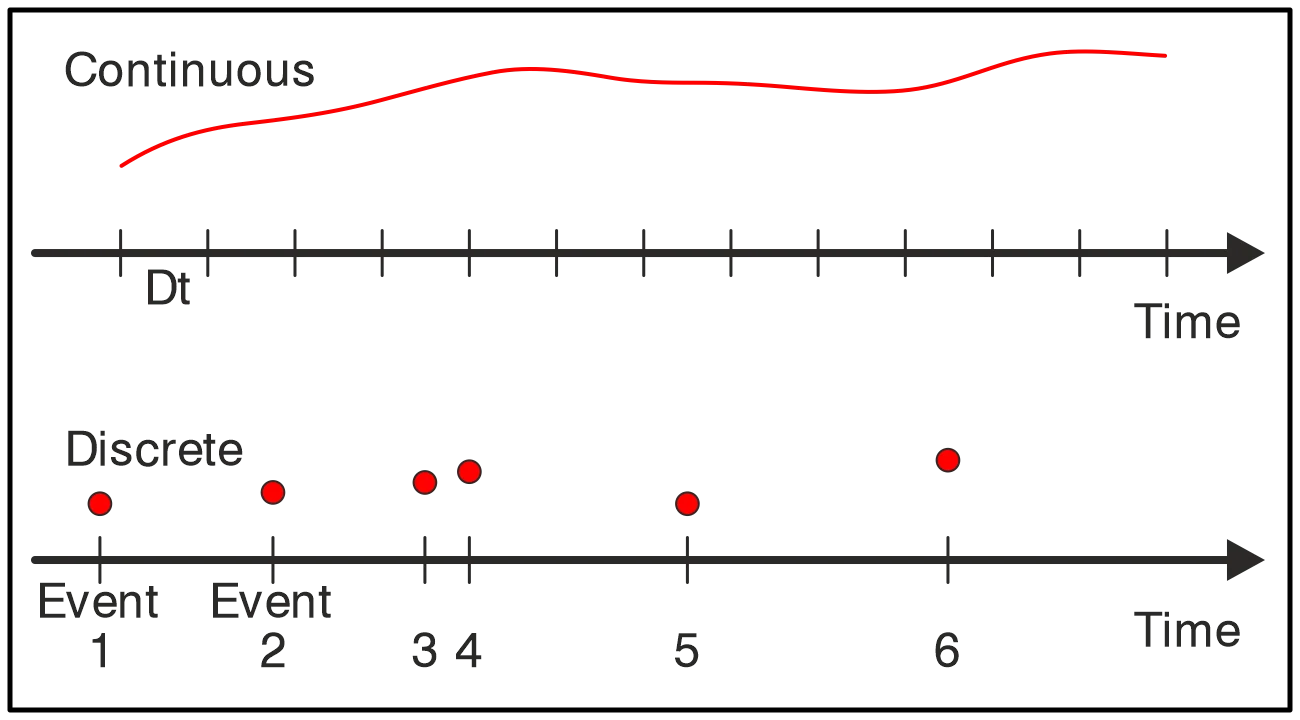
\includegraphics[width=.8\linewidth]{figures/discrete-event-simulation/Discrete-vs-Continuous-Simulation.png}
    \caption{Cambiamento di stato nel tempo in simulazioni continue vs simulazioni ad eventi discreti~\cite{Helal2008AHS}.}
    \label{fig:Continuous-vs-Discrete}
\end{figure}

Ad esempio, il livello dell'acqua in un serbatoio (la quale è una variabile di stato) può cambiare in modo continuo (ovvero con incrementi e decrementi infinitamente piccoli) e in qualsiasi punto del tempo continuo. Spesso questi modelli sono descritti da equazioni differenziali che specificano i tassi di variazione degli stati nel tempo.
Le simulazioni a tempo continuo non sono veramente continue nel senso matematico del termine poiché, per ragioni computazionali, è impossibile rappresentare il tempo in modo continuo su un computer. Anche se il concetto di tempo continuo è utilizzato nella modellazione e nella simulazione, il computer deve comunque discretizzare il tempo per eseguire le simulazioni in maniera efficiente e accurata.
Ci sono diverse ragioni per cui le simulazioni a tempo continuo non possono essere veramente continue:
\begin{itemize}
    \item limitazioni computazionali: i computer hanno una quantità finita di memoria e risorse di calcolo. Per simulare un processo continuo, il tempo deve essere discretizzato in intervalli finiti. Questo porta a una rappresentazione approssimata del tempo continuo, con una risoluzione determinata dalla precisione temporale della simulazione;
    \item errori numerici: anche con un elevato numero di punti discreti nel tempo, l'approssimazione del tempo continuo introduce errori numerici. Questi errori possono accumularsi nel tempo e influenzare l'accuratezza complessiva della simulazione;
    \item algoritmi di integrazione numerica: nelle simulazioni a tempo continuo, le equazioni differenziali che descrivono il sistema devono essere risolte numericamente utilizzando algoritmi di integrazione numerica, come ad esempio il metodo di Runge-Kutta. Questi algoritmi discretizzano implicitamente il tempo per calcolare l'evoluzione del sistema nel tempo.
\end{itemize}

In generale, poiché la simulazione in tempo continuo tiene traccia dello stato del sistema in modo continuo, è più granulare e, in certe situazioni (soprattutto nelle scienze naturali), più accurata. D'altra parte, la simulazione in tempo continuo può richiedere più risorse computazionali, perché il tracciamento continuo degli stati del sistema può essere costoso.

Un'altra differenza tra le simulazioni a tempo continuo e quelle ad eventi discreti è la loro adattabilità a problemi sia continui che discreti~\cite{zgn2009DiscreteVC}. Più precisamente:
\begin{itemize}
    \item la simulazione in tempo continuo può essere utilizzata per modellare processi continui e discreti. Sebbene i processi discreti non siano continui per natura, i modelli in tempo continuo possono modellarli con successo e generare risultati validi. Ad esempio, può succedere che fenomeni come il flusso del traffico di veicoli, siano approssimati da un modello a tempo continuo considerando il traffico come un fluido. Tuttavia, un modello in tempo continuo richiederebbe più tempo e calcoli per lo stesso problema discreto. Inoltre, per alcuni sistemi discreti, l'output di un modello di simulazione in tempo continuo potrebbe non avere senso.
    \item I modelli discreti potrebbero, in teoria, essere applicati anche ai sistemi a tempo continuo. Tuttavia, un modello a eventi discreti ne fornirebbe una visione meno raffinata, a causa della sua natura.
\end{itemize}

In conclusione, è preferibile utilizzare un modello ad eventi discreti quando: 
\begin{itemize}
    \item il sistema da modellare è caratterizzato da eventi distinti che influenzano il comportamento complessivo, come code di attesa, processi di produzione, reti di computer etc\dots
    \item il sistema mostra comportamenti che possono essere modellati efficacemente attraverso una serie di eventi distinti e continui; 
    \item le risorse computazionali sono limitate o gli eventi significativi sono rari nel tempo.
\end{itemize}
Mentre è da preferire la simulazione continua quando: 
\begin{itemize}
    \item il sistema è meglio descritto da equazioni differenziali o processi che si evolvono in modo continuo nel tempo, come sistemi meccanici, flussi di traffico o processi chimici; 
    \item è necessaria una rappresentazione accurata dei cambiamenti nel tempo, specialmente quando i dettagli più sottili del comportamento sono cruciali per l'analisi; 
    \item si dispone di risorse computazionali sufficienti per gestire la complessità richiesta.
\end{itemize}

\section{Simulazioni Time-Driven vs Event-Driven}
Esistono due tipi di simulazione discreta che possono essere distinti per quanto riguarda le politiche di avanzamento nel tempo all'interno della simulazione. In una simulazione discreta \textit{time-driven} il tempo simulato avanza in passaggi temporali (o \textit{ticks}) di dimensioni constanti $\Delta$, ovvero, l'osservazione del sistema dinamico simulato è discretizzata in intervalli di tempo unitari. La scelta di $\Delta$ determina la precisione della simulazione e il tempo di simulazione trascorso: i \textit{ticks} abbastanza brevi da garantire la precisione richiesta generalmente implicano un tempo di simulazione più lungo. Intuitivamente, per strutture event-driven irregolarmente distribuite nel tempo, l'approccio \textit{time-driven} genera algoritmi di simulazione inefficienti. 

La simulazione discreta con approccio \textit{event-driven} discretizza l'osservazione del sistema simulato negli istanti in cui si verificano gli eventi. Una simulazione ad eventi discreti, quando eseguita sequenzialmente, elabora ripetutamente l'occorrenza degli eventi nel tempo simulato, mantenendo una lista di eventi ordinata per tempo che tiene traccia degli eventi temporizzati programmati per accadere in futuro, un orologio globale che indica il tempo corrente e la variabili di stato $S = (s_1, s_2, \dots, s_n)$, che definiscono lo stato attuale del sistema. Come già descritto nella \Cref{sec:panoramica-des}, un motore di simulazione guida la simulazione prendendo continuamente il primo evento dalla lista degli eventi, simulando l'effetto dell'evento, cambiando le variabili di stato e eventualmente rimuovendo anche gli eventi obsoleti. Questo viene eseguito fino a quando viene raggiunto un tempo di fine predefinito, o non ci sono più eventi da verificarsi.

L'approccio \textit{event-driven} si concentra sulla relazione causale tra gli eventi esterni e le azioni eseguite da un sistema, ovvero sul \textbf{perché} accade qualcosa, mentre il modello \textit{time-driven} si concentra sul tempismo delle azioni, ovvero sul \textbf{quando} accade qualcosa. Nel primo caso, le azioni vengono eseguite \textbf{il prima possibile} all'arrivo degli eventi, e il tempo può essere gestito mediante segnali temporali trattati come eventi esterni asincroni. Al contrario, nel secondo caso le azioni vengono eseguite \textbf{al momento giusto} secondo un programma, e gli eventi esterni possono essere gestiti mediante meccanismi di polling~\cite{TISATO199531}.
La scelta tra i due modelli dipende dal dominio di applicazione. Nei sistemi complessi, i due modelli dovrebbero coesistere per soddisfare requisiti contrastanti. Di conseguenza, un linguaggio di programmazione dovrebbe consentire al progettista di scegliere e mescolare astrazioni per catturare nel modo più espressivo possibile i concetti chiave legati a un problema specifico o a un sotto-problema. 

\section{Simulatore Alchemist}

Alchemist~\cite{DBLP:journals/jos/PianiniMV13} è un simulatore ad eventi discreti open-source sviluppato all'interno dell'Università di Bologna, che permette la simulazione di scenari inerenti la computazione pervasiva ed ispirata alla natura. 
Alchemist si basa sull'algoritmo \textit{Next Reaction Method}~\cite{doi:10.1021/jp993732q}, un algoritmo di simulazione stocastica più efficiente dell'algoritmo di Gillespie~\cite{doi:10.1021/j100540a008}, su cui si basa.

\subsection{Modello del dominio}
Il dominio di Alchemist, rappresentato in~\Cref{fig:alchemist-model}, è rappresentato dalle seguenti entità: 
\begin{itemize}
    \item \textbf{Molecola}: il nome dei data item. Se Alchemist fosse un linguaggio imperativo, una molecola potrebbe rappresentare il nome di una variabile. 
    \item \textbf{Concentrazione}: il valore associato a una particolare molecola. In un linguaggio imperativo la concentrazione sarebbe il valore associato alla variabile. 
    \item \textbf{Nodo}: un contenitore di molecole e reazioni, che vivono all'interno di un environment. 
    \item \textbf{Environment}: è l'astrazione di Alchemist per lo spazio. È un contenitore di nodi con le seguenti funzionalità: 
    \begin{itemize}
        \item è capace di dirci dov'è un nodo nello spazio;
        \item è capace di dirci la distanza fra due nodi;
        \item opzionalmente ha il supporto per rimuovere i nodi.
    \end{itemize}
    \item \textbf{Regola di collegamento}: una funzione dello stato corrente dell'environment che associa ad ogni nodo un vicinato. 
    \item \textbf{Vicinato}: un'entità composta da un nodo e un insieme di nodi vicini. Il concetto di vicino deve essere il più generale e flessibile possibile: dal concetto fisico di agenti all'interno di un raggio, al concetto sociale di due agenti collegati da una relazione sociale di qualche tipo. 
    \item \textbf{Reazione}: il concetto di reazione è più elaborato di quello usato nella chimica: nei modelli classici, una reazione elenca un certo numero di molecole reagenti che, combinate, producono un insieme di molecole prodotto. In Alchemist una reazione è un evento capace di cambiare lo stato dell'environment. Ogni nodo ha un possibile insieme (anche vuoto) di reazioni. Ogni reazione è definita da una lista (anche vuota) di condizioni, una o più azioni ad essa associate e una distribuzione temporale. La frequenza con la quale accade dipende da:
    \begin{itemize}
        \item un parametro a tasso statico; 
        \item il valore di ciascuna condizione; 
        \item una distribuzione temporale
        \item un'equazione che a partire dal tasso statico e dai valori delle condizioni restituisce un tasso istantaneo.
    \end{itemize}
    Il suo funzionamento può essere osservato in~\Cref{fig:alchemist-reaction}
    \item \textbf{Condizione}: una funzione che prende come input l'environment corrente e restituisce in output un booleano. Per poter essere innescata, una reazione necessita che tutte le condizioni ad essa associate siano soddisfatte. Le condizioni sono tipicamente espresse come un elenco di annotazioni che devono essere disponibili in una località per l'esecuzione della reazione, ma possono anche includere considerazioni sulla forma del vicinato.
    \item \textbf{Azione}: modella i cambiamenti dell'environment. Le azioni possono essere la trasformazione, la rimozione o la produzione di annotazioni, lo spostamento di agenti, la duplicazione di essi e così via.
\end{itemize}

\begin{figure}
    \centering
    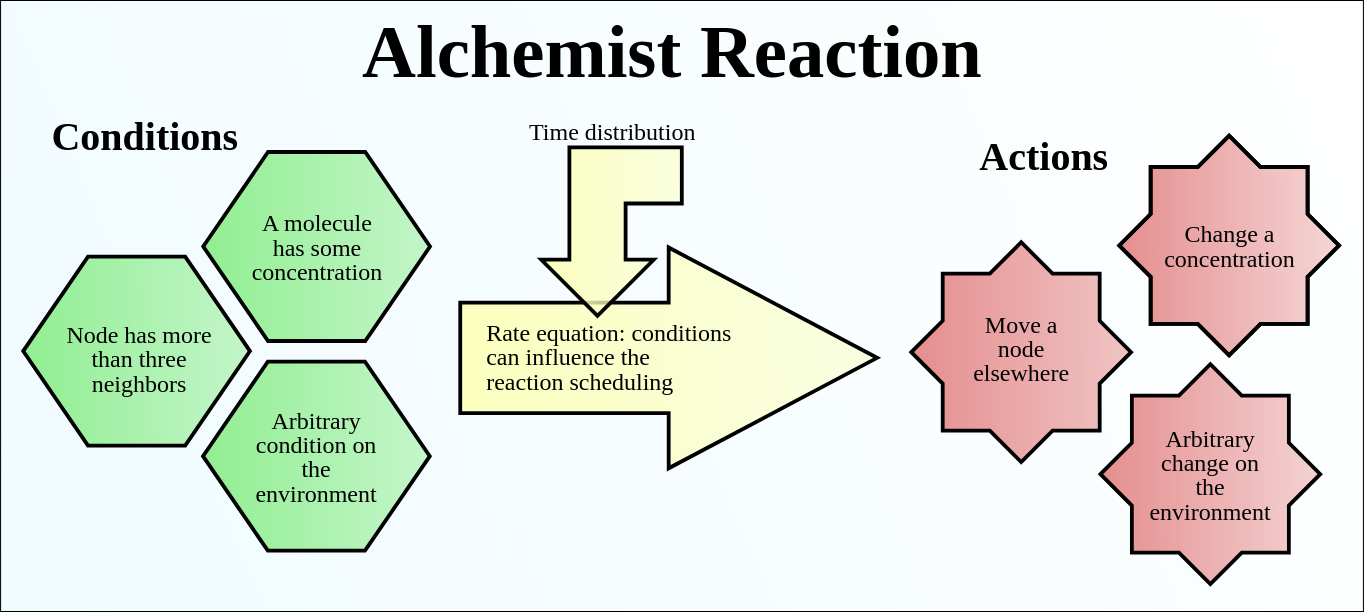
\includegraphics[width=.85\linewidth]{figures/discrete-event-simulation/alchemist-reaction.png}
    \caption{Rappresentazione grafica del funzionamento di una reazione}
    \label{fig:alchemist-reaction}
\end{figure}

\begin{figure}
    \centering
    \includegraphics[width=.85\linewidth]{figures/discrete-event-simulation/alchemist-model.png}
    \caption{Meta-modello alla base di Alchemist.}
    \label{fig:alchemist-model}
\end{figure}

Una delle caratteristiche principali del simulatore è la sua generalità. Essa viene raggiunta attraverso l'uso delle \textbf{incarnazioni}, ovvero le istanze concrete del meta-modello in cui ogni entità viene mappata ad un corrispettivo concetto dell'universo di interesse. 
Un'incarnazione di Alchemist include una definizione del tipo di concentrazione ed eventualmente un insieme di condizioni specifiche, azioni e (raramente) ambienti e reazioni che operano su tali tipi. 
Incarnazioni diverse possono modellare universi completamente diversi. Per esempio, come nel caso di \textbf{Biochemistry}, se la concentrazione viene definita come un numero intero positivo e vengono fornite azioni e condizioni adeguate, Alchemist diventa un simulatore stocastico di chimica con compartimenti interconnessi e mobili.
\textbf{SAPERE} è l'incarnazione più vecchia. In questa incarnazione le concentrazioni sono un insieme di tuple Linda-Like. È stata utilizzata per simulare evacuazione di folle, l'adattamento anticipato e l'esplorazione di risorse.  
Nel caso di \textbf{Protelis}, la concentrazione è definita come Java Object. In questa incarnazione i nodi eseguono specifiche scritte nel linguaggio Protelis~\cite{DBLP:conf/sac/PianiniVB15}. \textbf{Scafi} è dedicata alla programmazione aggregata ed è basata sul framework Scafi~\cite{DBLP:journals/softx/CasadeiVAP22}.

\subsection{Funzionalità e utilizzo del simulatore}
Per configurare una simulazione in Alchemist, è necessario fornire un file in formato YAML\footnote{https://yaml.org/}. Nel file di configurazione occorre specificare quali classi e parametri utilizzare. Le entità vengono identificate tramite chiavi, al livello zero è possibile trovare: 
\begin{itemize}
    \item \textbf{incarnation}: è l'unica chiave obbligatoria. Serve a specificare quale incarnazione si intende utilizzare; 
    \item \textbf{seed}: specifica il seme da utilizzare per generazione di numeri casuali. Questo serve a garantire la riproducibilità degli esperimenti scientifici. È essenziale, a fini di debug riuscire a garantire simulazioni sempre uguali partendo dalla stessa configurazione nel file YAML;
    \item \textbf{variables}: i valori che si intendono riutilizzare all'interno del file di configurazione. 
    \item \textbf{environment}: la tipologia di ambiente dentro al quale si intende eseguire la simulazione;
    \item \textbf{network-model}: permette di decidere come devono essere collegati fra loro i nodi;
    \item \textbf{export}: permette la configurazione e la scelta dei dati della simulazione che si intende esportare; 
    \item \textbf{deployment}: permette di definire quali sono i nodi del sistema e dove si trovano. 
\end{itemize}
Il simulatore può essere eseguito in due modalità: \textit{interattiva} o \textit{batch}. Nella prima viene eseguita una sola simulazione per volta mentre nella seconda vengono eseguite molteplici simulazioni che dipendono dai valori delle variabili impostati dall'utente. Impostando multipli valori per ciascuna variabile, il simulatore eseguirà una simulazione per ogni possibile combinazione di esse. 

Alchemist supporta il caricamento delle planimetrie e delle mappe geografiche. Il caricamento di una planimetria avviene a partire da un'immagine, convertendo i pixel adiacenti del colore specificato in ostacoli. Il supporto agli standard GPX e GPS rende invece possibile il caricamento di mappe. 
\subsection{Architettura}
Il framework, la cui architettura ad alto livello è osservabile in~\Cref{fig:alchemist-architecture}, è stato progettato per essere modulare ed estendibile. L'engine può essere re-implementato senza toccare niente del modello e il modello può essere esteso senza necessità di modificare l'engine. 

\begin{figure}
    \centering
    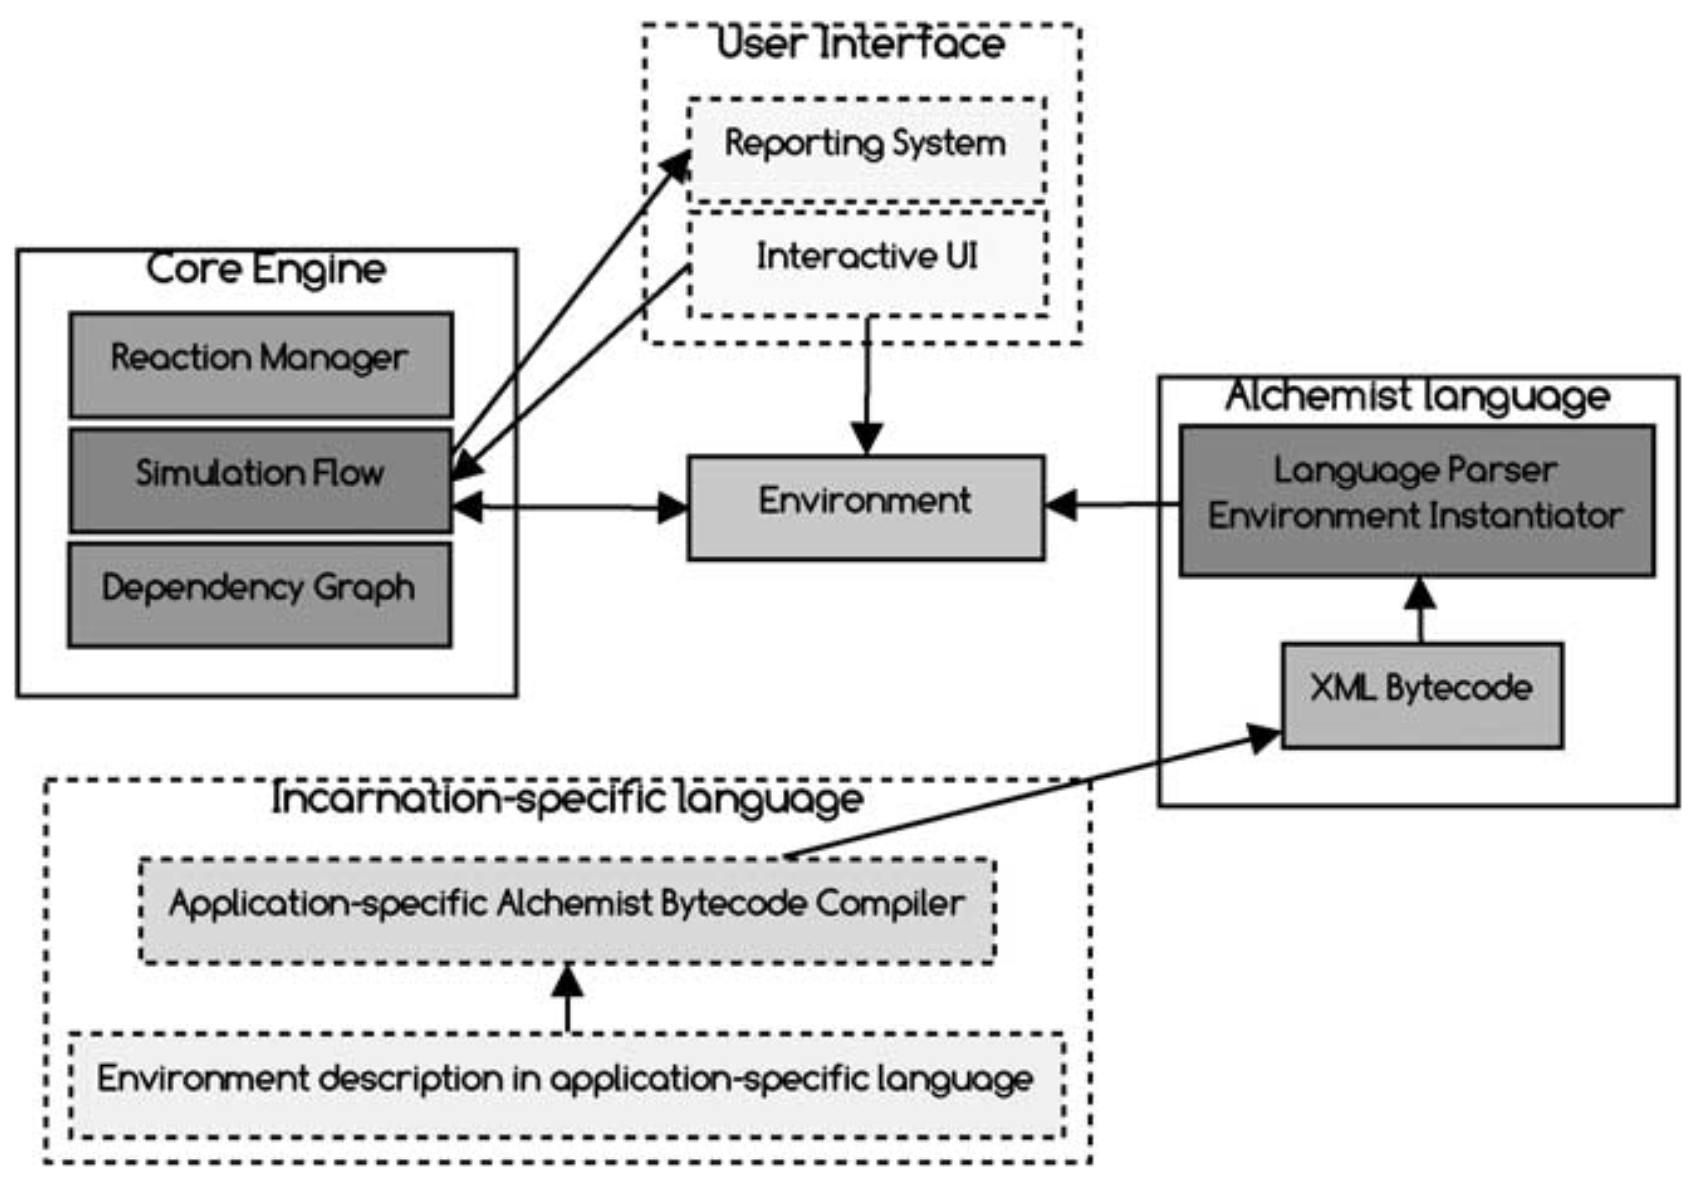
\includegraphics[width=.85\linewidth]{figures/discrete-event-simulation/alchemist-architecture.png}
    \caption{Architettura di Alchemist. Gli elementi disegnati con linee continue indicano i componenti comuni a tutti gli scenari, quelli con linee tratteggiate rappresentano componenti che devono essere sviluppati da una specifica incarnazione~\cite{DBLP:journals/jos/PianiniMV13}.}
    \label{fig:alchemist-architecture}
\end{figure}

\subsubsection{Engine}
Di seguito si intende descrivere brevemente il funzionamento dell'algoritmo \textit{Next Reaction Method}, utilizzato da Alchemist per selezionare il prossimo evento da eseguire e il \textit{Dynamic Dependency Graph}, utilizzato per gestire le dipendenze fra le reazioni presenti all'interno dei nodi. 
\paragraph{Next Reaction Method}
Come anticipato, Alchemist si basa sull'algoritmo di simulazione stocastica \textit{Next Reaction Method}. Ad ogni step della simulazione è in grado di selezionare la prossima reazione da eseguire in tempo costante. L'algoritmo richiede tempo logaritmico per aggiornare la struttura dati interna. L'algoritmo non sceglie la prossima reazione da eseguire valutando la sua velocità, ma generando un tempo putativo e ordinando le reazioni per decidere quale sia la prossima da eseguire. L'algoritmo originale è stato modificato per consentire di aggiungere, rimuovere o spostare le reazioni in modo dinamico. 
Le reazioni vengono memorizzate in una \textit{Dynamic Indexed Priority Queue}. Quest'ultima è un binary tree di reazioni, la sua proprietà principale è che ogni nodo memorizza una reazione il cui tempo di accadimento presunto è inferiore a quello di ciascuno dei suoi figli. Ciò significa che la prossima reazione da eseguire sarà sempre quella nella radice dell'albero e ci si potrà quindi accedere in tempo costante. 
Un'altra proprietà importante della \textit{priority queue} è che in assenza dell'aggiunta di nuovi nodi all'albero, lo swap fra due nodi non ne modifica il bilanciamento. 
In Alchemist i nodi vengono aggiunti e quindi non si riesce a sfruttare direttamente questa proprietà. L'idea è quindi di tenere traccia, per ogni nodo, del numero di discendenti per ogni ramo, avendo così la possibilità di mantenere bilanciato l'albero a seguito dell'aggiunta di nodi. 

\paragraph{Dynamic Dependency Graph}
Consiste in un grafo diretto, nel quale i nodi sono le reazioni e gli archi connettono una reazione $r$ a tutti i nodi che dipendono da essa, ovvero quelli il cui tempo di attivazione deve essere aggiornato a seguito dell'esecuzione di $r$. Per esempio, se $r$ muove una molecola da un nodo $n$ ad un nodo $m$, tutte le reazioni che usano le molecole in $m$ devono essere riprogrammate in modo appropriato non appena $r$ viene attivata.
Mantenere il grafo delle dipendenze aggiornato durante la simulazione è uno dei task più critici. Dato che si vuole supportare nativamente l'interazione fra nodi, che diventano dipendenze fra le reazioni che avvengono in questi nodi, sono definiti tre \textit{contesti} (chiamati anche \textit{scopes}): 
\begin{itemize}
    \item \textbf{locale}: la reazione influenza solo il nodo in cui avviene; 
    \item \textbf{vicinato}: la reazione influenza il suo nodo e tutto il vicinato; 
    \item \textbf{globale}: la reazione influenza tutte le altre reazioni. 
\end{itemize}
Ogni reazione ha un \textit{contesto di input}, ovvero il contesto più piccolo in cui una reazione può leggere informazioni, e un \textit{contesto di output}, ovvero il contesto più piccolo nel quale una reazione può effettuare modifiche. 
La scelta del contesto giusto è cruciale: se è troppo ristretto la simulazione sarà invalida, se viene scelto troppo grande, questo impatterà pesantemente sulle performance. 
L'aggiunta di una reazione implica la verifica delle sue dipendenze con tutte le reazioni del sistema. Se esiste, questa dipendenza viene aggiunta al grafo delle dipendenze. La rimozione di una reazione richiede l'eliminazione di tutte le dipendenze in cui quest'ultima è coinvolta, sia come influenzante che come influenzata. 
In caso di cambiamento della topologia del sistema è necessario un ulteriore controllo delle dipendenze tra le reazioni appartenenti ai nodi che hanno subito un cambiamento del proprio vicinato. Occorre eseguire una scansione in questi nodi, calcolando le nuove dipendenze con le reazioni appartenenti ai nuovi vicini e cancellando quelle con i nodi che non appartengono più al vicinato. 

\chapter{Programmazione reattiva}
\section{Concetti chiave della programmazione reattiva}
\subsection{Definizione}
L'uso del termine programmazione reattiva nella letteratura scientifica risale alla metà degli anni '60. Una definizione rilevante è stata data da G. Berry nel 1991~\cite{DBLP:journals/pieee/BenvenisteB91}. Berry descrive i programmi reattivi in relazione alla loro controparte duale, i programmi interattivi: 
\begin{quotation}
    "I programmi interattivi interagiscono alla propria velocità con gli utenti o con altri programmi; dal punto di vista dell'utente, un sistema time-sharing è interattivo. Anche i programmi reattivi mantengono una continua interazione con l'ambiente, ma a una velocità che è determinata dall'ambiente e non dal programma stesso"
\end{quotation}

I programmi interattivi concretizzano l'idea di un modello di calcolo ``pull-based'', in cui il programma - in questo caso il consumatore - ha il controllo sulla velocità con cui i dai vengono richiesti e gestiti. 
Un esempio perfetto di programma interattivo è una struttura di flusso di controllo come un ciclo for che itera su un insieme di dati: il programma ha il controllo della velocità con cui i dati vengono recuperati dalla collezione e richiederà l'elemento successivo solo aver terminato la gestione di quello attuale. 

I programmi reattivi, al contrario, incarnano l'idea di un modello di calcolo ``push based'', in cui la velocità con il programma interagisce con l'ambiente è determinata dall'ambiente stesso piuttosto che dal programma. In altre parole, ora è il produttore dei dati a determinare la velocità con cui si verificheranno gli eventi, mentre il ruolo del programma si riduce a quello di un osservatore silenzioso che reagisce alla ricezione degli eventi. Esempi standard di tali sistemi sono le applicazioni GUI che si occupano di vari eventi originati dall'input dell'utente, come per esempio il click del mouse. Queste applicazioni sono difficili da programmare con i tradizionali approcci di programmazione sequenziale, perché è impossibile prevedere o controllare l'ordine di arrivo degli eventi esterni. Inoltre quando si verifica un cambiamento di stato in un calcolo o in un dato, il programmatore deve aggiornare tutti gli altri che dipendono da esso. Questa gestione manuale dei cambiamenti di stato e delle dipendenze dei dati è complessa e soggetta ad errori.

Utilizzando soluzioni di programmazione tradizionali, le applicazioni interattive sono tipicamente costruite attorno alla nozione di callback asincrone. 
Coordinare le callback può essere un compito arduo, poiché numerosi frammenti di codice isolati possono manipolare gli stessi dati e il loro ordine di esecuzione non è prevedibile. Inoltre, le callback solitamente non hanno un valore di ritorno, quindi sono richiesti side-effect per modificare lo stato dell'applicazione~\cite{DBLP:phd/us/Cooper08}. 

Il paradigma della programmazione reattiva è stato recentemente proposto come soluzione adatta allo sviluppo di applicazioni event-driven. La programmazione reattiva affronta i problemi posti dalla applicazioni event-driven fornendo astrazioni per esprimere i programmi come reazioni a eventi esterni e facendo in modo che il linguaggio gestisca automaticamente il flusso del tempo e le dipendenze di dati e calcoli. Ciò comporta il vantaggio che i programmatori non devono preoccuparsi dell'ordine degli eventi e delle dipendenze di calcolo. I linguaggi di programmazione reattivi astraggono dalla gestione del tempo, proprio come i garbage collector astraggono dalla gestione della memoria. 

\subsection{Propagazione del cambiamento}
La programmazione reattiva è un paradigma che si basa sulla nozione di valori variabili e continui nel tempo e sulla propagazione del cambiamento. 
In questo paradigma i cambiamenti di stato vengono automaticamente ed efficientemente propagati attraverso la rete di computa<ioni dipendenti dal modello di esecuzione sottostante. Consideriamo un semplice esempio di calcolo della somma di due variabili.
\begin{quotation}
    \texttt{var1 = 1}
    \texttt{var2 = 2}
    \texttt{var3 = var1 + var2}
\end{quotation}

Nella programmazione sequenziale imperativa convenzionale il valore della variabile \texttt{var3} conterrà sempre il valore 3, ovvero la somma dei valori iniziali delle variabili \texttt{var1} e \texttt{var2}.
Nella programmazione reattiva il valore di \texttt{var3} è sempre aggiornato perché viene ricalcolato ogni volta che il valore di \texttt{var1} o \texttt{var2} cambia.
Questa è la nozione chiave della programmazione reattiva. I valori cambiano nel tempo e tutti i calcoli dipendenti vengono automaticamente rieseguiti. Nella terminologia della programmazione reattiva la variabile \texttt{var3} è detta dipendente dalle variabili \texttt{var1} e \texttt{var2}. La dipendenza in questione può essere osservata in~\Cref{fig:rp-dependency}.

La logica della propagazione del cambiamento può essere implementata per mezzo di un grafo i cui nodi rappresentano i valori da tenere aggiornati e gli archi rappresentano le relazioni di dipendenza che coinvolgono i nodi. Utilizzando questo tipo di architettura si viene quindi a creare una rete di dipendenze computazioni ed il cambiamento di un nodo (quindi di un valore) scatena una reazione che implica l'attraversamento degli eventuali archi ad eso collegati e il conseguente aggiornamento di tutti i nodi raggiunti. 

\begin{figure}
    \centering
    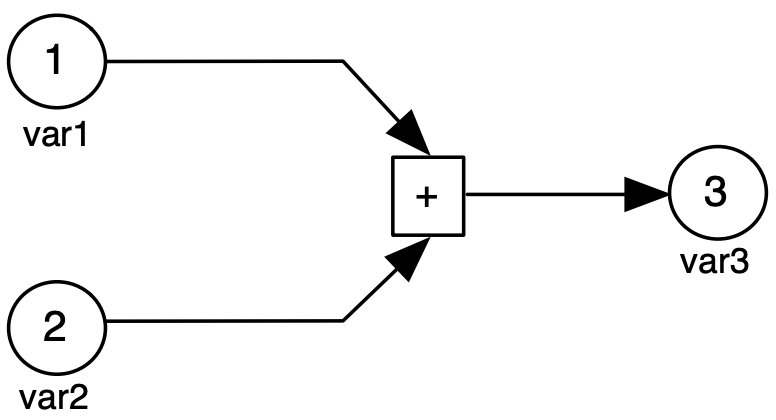
\includegraphics[width=.65\linewidth]{figures/reactive-programming/RP-dependency.png}
    \caption{Rappresentazione grafica della dipendenza fra espressioni nella programmazione reattiva \cite{DBLP:journals/csur/BainomugishaCCMM13}.}
    \label{fig:rp-dependency}
\end{figure}

\subsubsection{Strategie di propagazione}
Esistono diverse strategie adottabili per la propagazione del cambiamento nella programmazione reattiva, di seguito verranno descritte le principali:
\begin{itemize}
    \item \textbf{complete propagation}: ogni nodo, durante la propagazione, invia il suo stato attuale completo ai nodi dipendenti. In questo caso tutto lo stato precedente del nodo viene perso durante l'aggiornamento del nuovo stato. Questa strategia non è adatta nei casi in cui il grafo delle dipendenze sia particolarmente complesso o nel caso in cui gli stati necessitino di grandi quantità di dati per essere descritti a causa del suo alto carico computazionale;
    \item \textbf{delta propagation}: al momento della propagazione i nodi interrati inviano solo una porzione (un \textit{delta}) del loro stato ai nodi dipendenti, cioè solo le frazioni di informazioni che sono state effettivamente coinvolte da modifiche. Questo approccio tende a minimizzare la quantità di dati da trasportare lungo la catena di dipendenze durante la propagazione dei cambiamenti, dunque risulta efficiente anche nei casi in cui si ha un grafo delle dipendenze complesso e una grande quantità di dati per la rappresentazione degli stati; 
    \item \textbf{batch propagation}: prevede un ritardo nella propagazione dei cambiamenti, cioè la rappresentazione ritardata nel tempo. Consente l'ottimizzazione di quelle situazioni in cui abbiamo più cambiamenti vicini nel tempo che si annullano a vicenda e fanno sì che si ritorni allo stato di partenza. Nel caso in cui due o più cambiamenti vicini nel tempo generino un'effettiva mutazione di stato nel grafo viene propagato solo l'ultimo cambiamento, scartando i precedenti, ormai obsoleti. Questa strategia tende a minimizzare il numero di propagazioni e di conseguenza il carico computazionale complessivo. 
    Tuttavia, occorre adottare un tempo di ritardo corretto, al fine di ridurre il carico computazionale ma al tempo stesso garantire una buona reattività; 
    \textbf{invalidity notification propagation}: potrebbe essere definita come una "sotto-strategia" piuttosto che ua vera e propria strategia implementativa. Consiste nella richiesta di aggiornamento da parte di un nodo che riscontra di possedere uno stato non valido, oppure che riceve un messaggio di propagazione non valido. In questo caso il nodo interessato scarta l'anomalia e richiede ai nodi da cui dipende un nuovo aggiornamento. 
\end{itemize}

\subsection{Modelli di valutazione}
Nella programmazione reattiva, per \textit{modello di valutazione} (\textit{evaluation model}) si intende la dinamica direzionale che viene adottata per gestire la propagazione dei cambiamenti nel grafo delle dipendenze computazionali. 
Il modello viene applicato a livello di linguaggio, rimanendo quindi trasparente all'utilizzatore finale. 
I modelli presenti in letteratura sono due, ai quali si aggiunge un terzo, ibrido fra i primi due: 
\begin{itemize}
    \item \textbf{push-based}: nel modello push-based la reazione inizia quando un nodo produttore cambia stato aggiornandosi. Il nodo in questione ``spinge'' l'informazione attraverso i nodi consumatori, ovvero i nodi dipendenti. Questo approccio, guidato dalla disponibilità di nuove informazioni, ha il vantaggio di rendere il sistema altamente reattivo, in quanto le reazioni vengono provocate e propagate immediatamente dopo la disponibilità di nuovi dati. Questo approccio comporta, d'altra parte, a computazioni superflue e un alto carico di calcolo, a causa delle elaborazioni necessarie ad ogni cambiamento di stato del produttore. 
    \item \textbf{pull-based}: nel modello pull-based sono i nodi consumatori a richiedere i nuovi valori nel momento in cui ne hanno bisogno. L'approccio in questo caso è guidato dalla domanda di nuovi dati da parte dei nodi dipendenti. Questo porta ad un sistema più flessibile, ma introduce latenze fra il momento in cui un cambiamento si verifica e il momento in cui avviene la reazione. 
    \item \textbf{hybrid push-pull}: il modello ibrido combina i due modelli push e pull, cercando di trarre i vantaggi di entrambe le soluzioni. Il modello push-based funziona bene quando è richiesta una reazione istantanea al cambiamento, mentre il modello pull-based porta a prestazioni migliori quando nel sistema si presentano continui cambiamenti di valori nel tempo. Questo approccio riesce quindi a trarre i benefici del modello push-based (efficienza e latenza bassa) e del modello pull-based (flessibilità nella richiesta dei valori)~\cite{DBLP:conf/haskell/Elliott09}.  
\end{itemize}


\subsection{Glitch}
In programmazione reattiva un \textbf{glitch} indica un malfunzionamento dovuto ad una inconsistenza dei dati presenti nel grafo delle dipendenze computazionali. La prevenzioni dei glitch è un'altra proprietà che deve essere presa in considerazione in un linguaggio reattivo~\cite{DBLP:journals/csur/BainomugishaCCMM13}.
Un glitch può essere provocato da una anomalia durante la propagazione di un cambiamento, oppure dal calcolo di un espressione presente in un nodo prima della valutazione di tutte le sue dipendenze. Il risultato è una situazione nella quale un nodo esegue la propria computazione utilizzando alcuni dati aggiornati ed altri ormai obsoleti, provocando quasi certamente errori di calcolo e inconsistenze. 
Consideriamo il seguente esempio: 
\begin{quotation}
    \texttt{var1 = 1}
    \texttt{var2 = var1 * 1}
    \texttt{var3 = var1 + var2}
\end{quotation} 
In questo esempio, il valore della variabile \texttt{var2} dovrebbe essere sempre lo stesso di \texttt{var1}, e il valore di \texttt{var3} dovrebbe invece essere il doppio di \texttt{var1}. Inizialmente quando il valore di \texttt{var1} è 1, il valore di \texttt{var2} è 1, e quello di \texttt{var3} è 2. Se il valore di \texttt{var1} cambia, per esempio diventa 2, ci si aspetta che il valore di \texttt{var2} diventi 2 e di conseguenza quello di \texttt{var3} diventa 4. Tuttavia, in una implementazione reattiva non corretta, il cambiamento del valore di \texttt{var1} potrebbe causare il ricalcolo di \texttt{var1 + var2} prima di \texttt{var1 * 1} . In questo caso il valore di \texttt{var3} sarebbe momentaneamente 3, ovvero un valore non corretto.
Prima o poi l'espressione \texttt{var1 * 1} sarà computata, in quel momento il valore di var2 diventerà 2 e quello di var3 sarà ricalcolato, riflettendo il valore corretto 4. Il comportamento appena descritto è osservabile in 

\begin{figure}
    \centering
    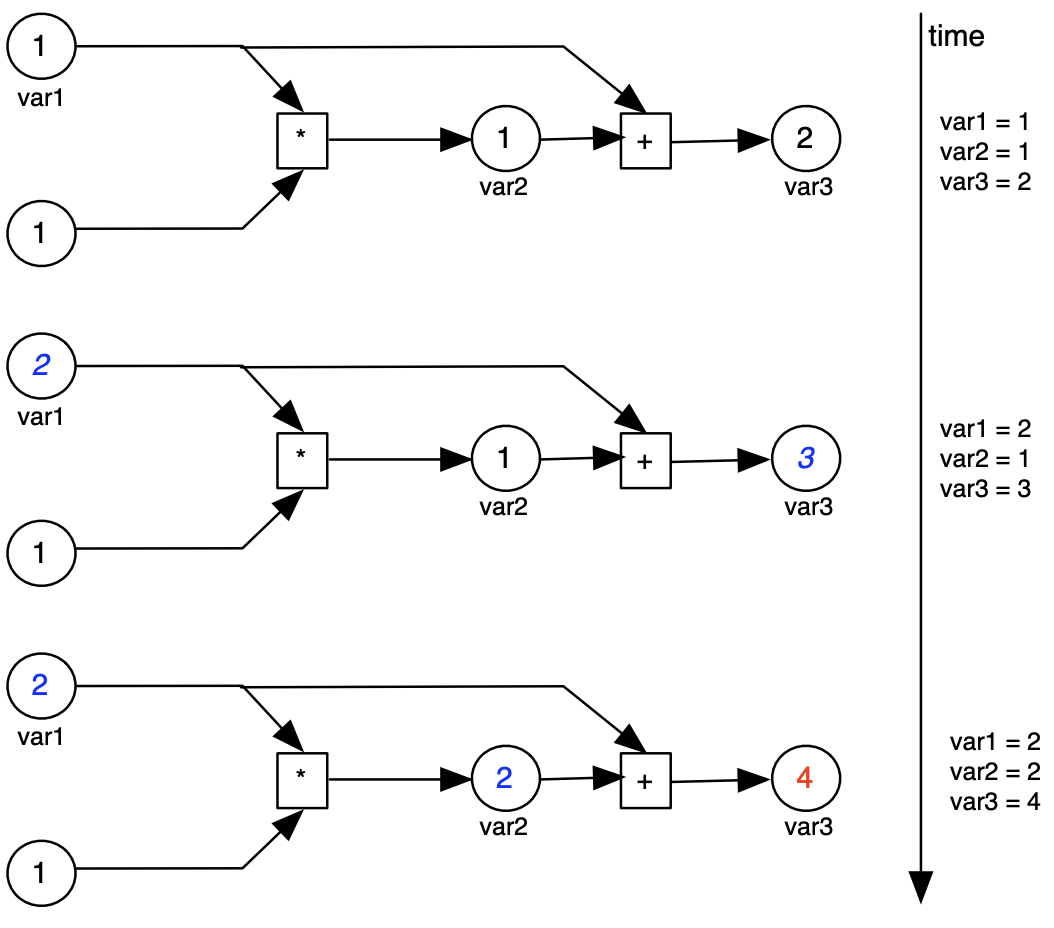
\includegraphics[width=.65\linewidth]{figures/reactive-programming/RP-glitch.png}
    \caption{Rappresentazione di un possibile glitch nella programmazione reattiva \cite{DBLP:journals/csur/BainomugishaCCMM13}.}
    \label{fig:rp-glitch}
\end{figure}

La maggior parte dei linguaggi di programmazione reattiva elimina i glitch organizzando le espressioni in un grafico ordinato topologicamente, garantendo così che un'espressione venga sempre valutata dopo che tutte le dipendenze sono state valutate. 
Nella teoria dei grafi l'ordinamento topologico di un grafo consiste nell'ordinare linearmente i suoi nodi in modo che preso un qualunque arco $xy$ dal nodo $x$ al nodo $y$, $x$ venga prima di $y$ nell'ordinamento. In altre parole, i nodi sono disposti in modo tale che ognuno di essi preceda tutti i nodi collegati ai suoi archi uscenti seguendo l'ordinamento scelto.
Le implementazioni reattive più recenti riescono ad evitare i glitch nei programmi reattivi eseguiti su un singolo computer, ma non nei programmi reattivi distribuiti. Evitare problemi in un ambiente distribuito non è un'attività banale a causa dei guasti di rete, ritardi e mancanza di un orologio globale. 

\subsection{Lifting}
Quando la programmazione reattiva è incorporata nei linguaggi host (come libreria o come estensione), gli operatori esistenti (ad esempio + o *) e le funzioni o i metodi definiti dall'utente devono essere convertiti per operare sui comportamenti. 
La conversione di un operatore ordinario in una variante in grado di operare sui comportamenti è nota come \textit{lifting}. 
Il lifting ha un duplice scopo: trasforma la firma del tipo di una funzione e registra un grafico delle dipendenze nel grafico del flusso di dati dell'applicazione. 
Esistono diverse strategie per effettuare il lifting: 
\begin{itemize}
    \item \textbf{lifting implicito}: quando un operatore viene applicato ad un comportamento, viene eseguito in maniera automatica il lifting. Il lifting implicito rende la programmazione reattiva trasparente agli utilizzatori. 
    \item \textbf{lifting esplicito}: in questo caso il linguaggio fornisce una serie di combinatori che possono essere utilizzati per effettuare il lifting.
    \item \textbf{lifting manuale}: il linguaggio non fornisce operatori per effettuare il lifting. Il programmatore deve ottenere manualmente il valore corrente di un valore variabile nel tempo, che poi può essere utilizzato con gli operatori del linguaggio. 
\end{itemize}

\subsection{Entità osservabili e osservatrici}
Nel contesto della programmazione reattiva, le fonti di dati o eventi che emettono informazioni vengono chiamate entità osservabili, mentre le entità osservatrici sono quelle che si collegano a queste fonti per monitorare e reagire ai dati o agli eventi emessi. In questa sezione vengono descritte le due entità, evidenziando le loro caratteristiche. 
\subsubsection{Entità osservabile}
Un'entità osservabile rappresenta un flusso continuo di dati o eventi che può essere emesso in modo regolare o completamente asincrono. Questo flusso può essere caratterizzato da una quantità variabile di elementi, incluso zero, uno o un numero infinito di essi. Questo concetto è fondamentale per gestire dati in tempo reale e interazioni utente in applicazioni moderne, consentendo una gestione dinamica dei flussi di informazioni.

Tuttavia, l'entità osservabile va oltre la semplice emissione di dati o eventi. Essa può concludersi in due modi principali: notificando un completamento avvenuto o segnalando un errore anomalo durante la sua esecuzione. Il completamento avvenuto è tipicamente utilizzato quando il flusso di dati ha termini definiti e finiti, ad esempio dopo il completamento di una sequenza di operazioni. D'altra parte, l'errore può essere segnalato in caso di malfunzionamenti imprevisti, come errori di connessione di rete o eccezioni di programmazione.

Se consideriamo un'entità osservabile con un flusso infinito di elementi, come ad esempio gli eventi di click dell'utente in un'applicazione Android, è importante notare che non sarà mai in grado di emettere un messaggio di completamento. Questo perché il completamento è riservato solo al termine naturale del flusso di eventi disponibili, il quale, se infinito, non si verifica mai. Tuttavia, è possibile che l'entità osservabile termini in modo anomalo, segnalando un errore, nel caso si verifichino anomalie durante la sua esecuzione. In tal caso, l'entità osservabile con un flusso infinito terminerà anticipatamente e non emetterà ulteriori elementi.

\subsection{Entità Osservatrice}
Un'entità osservatrice può instaurare una connessione (sottoscrizione) con un'entità osservabile al fine di monitorare e gestire i dati o gli eventi trasmessi da quest'ultima secondo specifiche politiche reattive. 
Gli elementi all'interno di un flusso sono emessi in modo sequenziale, uno dopo l'altro, e vengono elaborati dall'entità osservatrice in modo consecutivo. Questa caratteristica impedisce la comparsa di corse critiche, mantenendo l'ordine delle operazioni e garantendo una gestione reattiva dei dati.
Nel caso in cui un grande numero di dati o eventi venga emesso rapidamente dall'entità osservabile e l'entità osservatrice non sia in grado di elaborarli con la stessa velocità, è possibile adottare strategie come l'utilizzo di una coda degli eventi o il meccanismo di buffering per gestire in modo efficiente il flusso di dati e prevenire perdite o sovraccarichi.
Infine, un'entità osservabile può essere sottoscritta da zero, una o più entità osservatrici contemporaneamente, permettendo una gestione flessibile e dinamica del flusso di dati o eventi all'interno di un'applicazione reattiva. 
\subsection{Contesti di utilizzo}

\subsection{Il manifesto reattivo}
%----------------------------------------------------------------------------------------
% BIBLIOGRAPHY
%----------------------------------------------------------------------------------------

\backmatter

%\nocite{*} % comment this to only show the referenced entries from the .bib file

\bibliographystyle{alpha}
\bibliography{bibliography}

\end{document}